%Compiler avec pdflatex, le résultat ne doit pas dépasser une page
%Merci de respecter scrupuleusement ce modèle.
\documentclass[a4paper,titlepage,12pt,normalheadings,makeidx]{article}

\usepackage{graphicx} 
\usepackage[utf8]{inputenc}
\usepackage[francais]{babel}

\begin{document}
\newpage

% Titre
\subsection*{C. Bazgan et P. Beaujean: Modèle de résumé pour JGA}

% Sommaire
\addcontentsline{toc}{section}{C. Bazgan et P. Beaujean : Modèle de résumé pour JGA}

% Liste des auteurs (l'orateur est souligné) 
Cristina Bazgan, LAMSADE, Paris,
\texttt{cristina.bazgan@lamsade.dauphine.fr}\\
\indent
\underline{Paul Beaujean}, LAMSADE, Paris,
\texttt{paul.beaujean@lamsade.dauphine.fr}\\
\\

% Corps du résumé
Veillez à ce que le résumé n'excède pas {\bf 1 page}. Ne réduisez pas la taille
de la police.

Si vous souhaitez ajouter une image, faîtes en sorte qu'elle soit compilable
par \texttt{pdflatex} (pas de \texttt{pstricks} ou d'\texttt{eps}).
Vous pouvez aussi utiliser des images au format PDF ou PNG.

% Figure au format PDF ou PNG (facultatif)
\begin{figure}[ht]
\begin{center}
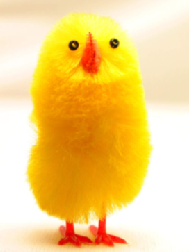
\includegraphics[height=3cm]{../img/chick.png}
\caption{Exemple de figure \label{Fig:chick}}
\end{center}
\end{figure}
\vfill
\end{document}
